\documentclass{article}

\usepackage{caption,color,fancyvrb,subfig}
\usepackage{code,algorithmic,algorithm}
%\usepackage{graphicx,epsfig}
\usepackage{amsmath,amsthm,amsfonts}
%\usepackage{url}
\usepackage{graphicx}
\usepackage{setspace}
\usepackage{bibentry}
 \nobibliography{prelim}

\textwidth = 6.5 in
\textheight = 9 in
\oddsidemargin = 0.0 in
\evensidemargin = 0.0 in
\topmargin = 0.0 in
\headheight = 0.0 in
\headsep = 0.0 in
\parskip = 0.2in
\parindent = 0.0in

\def\inv{^{-1}}


\begin{document}



\begin{titlepage}
\begin{center}

\textsc{\huge \bfseries \sc{Responsive Consistency in Heterogenous,}}\\
\textsc{\huge \bfseries \sc{Wide Area Distributed Storage Systems}}\\[1.0cm]

\emph{A prospectus submitted in partial fulfillment of the degree of Doctor of
Philosophy}\\[5.5cm]

\textsc{\large DRAFT}\\
\emph{October 11, 2016}\\[2.0cm]

\emph{Preliminary Oral Examination for}\\
\textsc{\large Benjamin Bengfort}\\[2.0cm] % [4.0cm]
\emph{Advisor:} \\
\textsc{Dr. Peter J. Keleher}\\[.5cm]
\emph{Committee Members:}\\
\textsc{Dr. Bobby Bhattacharjee}\\
\textsc{Dr. Dave Levin}\\
\textsc{Dr. Neil Spring}\\[4.0cm]

{\bfseries Department of Computer Science}\\
{\bfseries University of Maryland, College Park, MD 20742}\\
{\bfseries December 9, 2016}
\vfill

\end{center}
\end{titlepage}

\newpage
\thispagestyle{empty}
\mbox{}


\newpage
\setcounter{page}{1}
\doublespacing
\begin{abstract}

Data-oriented consistency is not a discrete set of various levels, weak, eventual, causal, strong etc. but rather a continuum that can be adapted in response to environmental conditions. Recent studies of consistency have focused on data center environments which are low latency, high bandwidth, and generally stable; and as a result data distribution involves a relatively small network of devices. I propose to study consistency in a user-oriented context composed of heterogenous devices (mobile phones, desktops, laptops, cloud storage) that can be mobile, creating a network topology of highly variable latency with routine failure and whose networks are larger than typically studied - dozens to hundreds of replica servers.

Our primary context will be a file system that exposes close-to-open consistency and tracks writes to individual objects as a sequence of versions structured as a tree. We consider strong consistency to be a linear sequence of ordered version numbers and inconsistencies to be the presence of forks, misordering, duplicates, or omissions in the version sequence (in order of severity). Additionally we consider the availability of such a system and recognize that enforcement of a linear ordering leads to high latency making the system unusable.

I propose that consistency is primarily related to the network environment as much as it is related to the implemented protocol and as a result, that it can respond the the environment. By creating a system that has a strong central core that maintains a globally consistent view and allowing other replica servers to be flexible I hypothesize that the system will be more consistent than its homogeneous counterparts reducing the number of forks, misordering, duplicates, and omissions as well increasing the throughput and availability of accesses in the system. I propose two primary mechanisms to make this happen:

\begin{enumerate}
    \item \textbf{Hierarchical Consensus}: distribute consensus decisions of sequential ordering in order to make stronger consistency more available.
    \item \textbf{Federated Consistency}: allow multiple consistency models for different replica servers, integrating over different aspects: temporal, spatial, and synchronization to create a flexible topology of devices with different characteristics and nodes.
\end{enumerate}

The experimentation on and development of multi-modal replication protocols via a holistic view will have a large impact in both the data center context as well as in personal distributed file systems.

\end{abstract}
\setstretch{.5}

\newpage
\tableofcontents

\newpage
\listoffigures

\newpage
\doublespacing

%\begin{figure}[!h]
%\begin{center}
%\begin{verbatim}
%/* Sample code snippet */
%\end{verbatim}
%\end{center}
%\caption{Code snippet caption}
%\label{fig:sample_code}
%\end{figure}

% \begin{figure}[!h]
%     \centering
%         \includegraphics[width=.9\textwidth]{figures/figure.png}
%         \caption{Figure caption}
%         \label{fig:label}
% \end{figure}

\section{Introduction}





\section{Related Work}

\subsection{Consistency}

\subsection{Anti-Entropy}

\subsection{Consensus}

\subsection{Systems}

\subsubsection{Bayou}

\subsubsection{SUNDR}

\subsubsection{Camlistore}

\subsubsection{OriFS}

\subsubsection{Stellar}

\section{Preliminary Work}

\subsection{Topology}

\begin{figure}[!h]
    \centering
        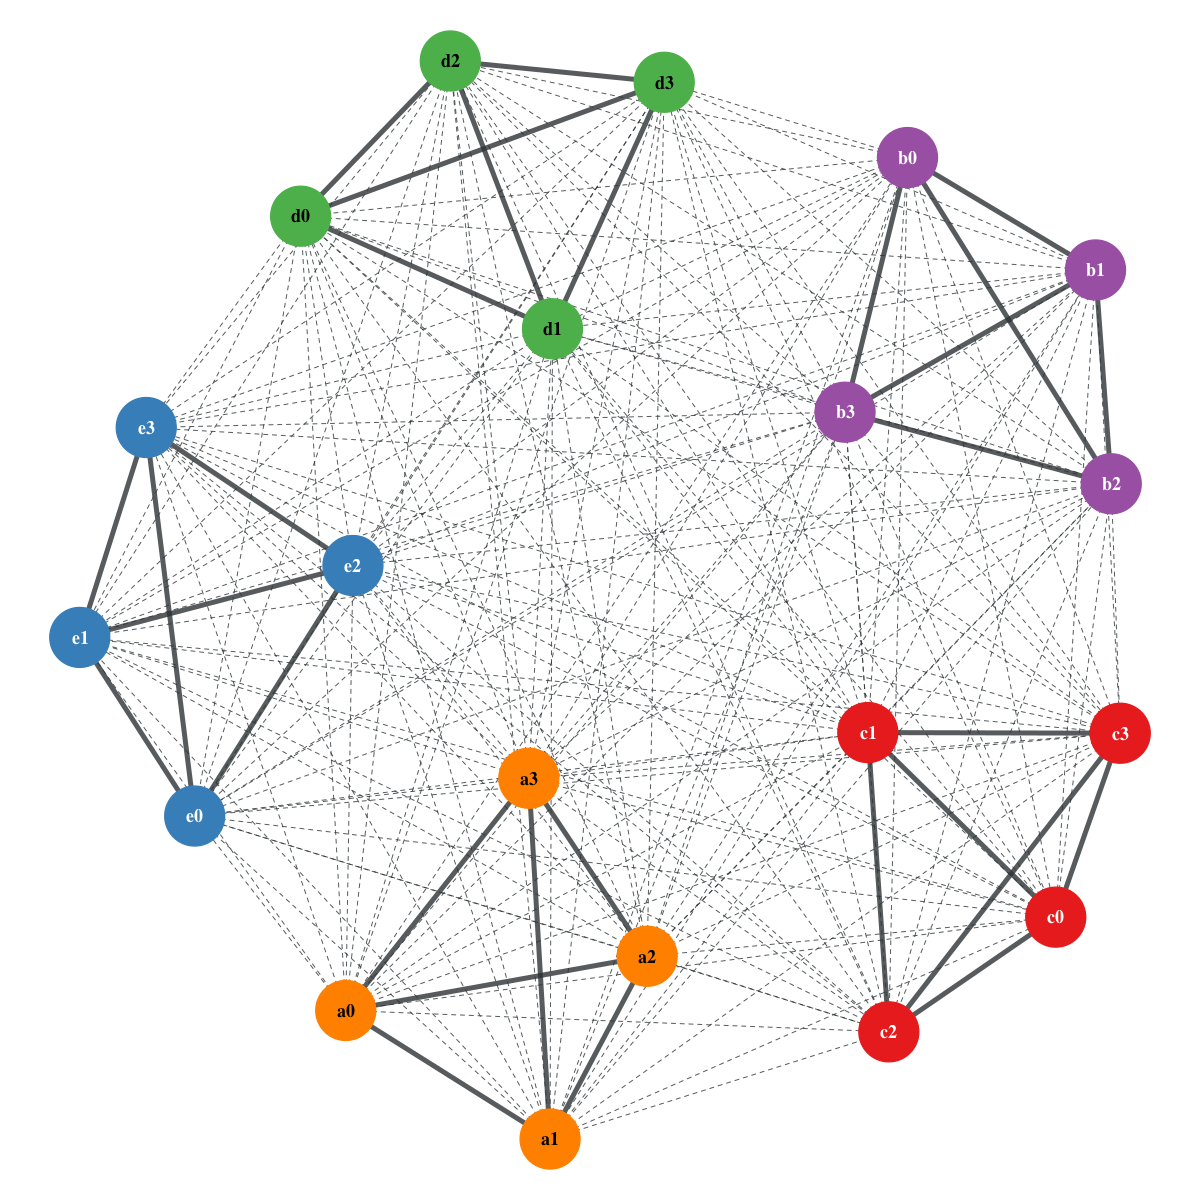
\includegraphics[width=.9\textwidth]{figures/topology}
        \caption{Proposed topology}
        \label{fig:topology}
\end{figure}

\subsection{System Description}

\begin{figure*}[!h]
    \centering
    \minipage{0.5\textwidth}
      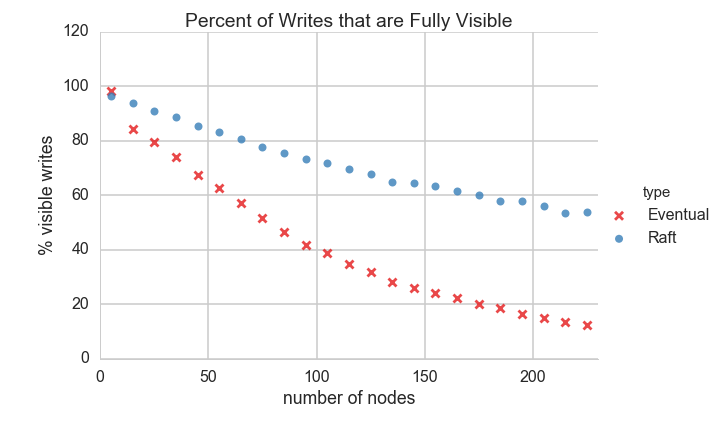
\includegraphics[width=\linewidth]{figures/scaling/visible_writes}
      \caption{Percent versions that become fully replicated.}\label{fig:scaling_visible_writes}
    \endminipage\hfill
    \minipage{0.5\textwidth}
      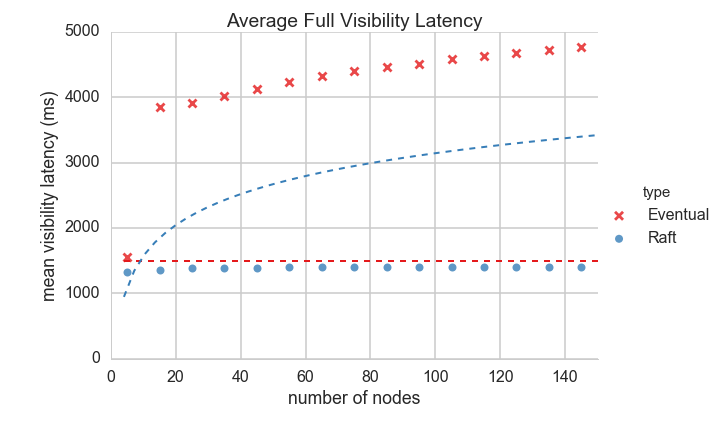
\includegraphics[width=\linewidth]{figures/scaling/visibility_latency}
      \caption{Time to full visibility.}\label{fig:scaling_visibility_latency}
    \endminipage
\end{figure*}

\begin{figure*}[!h]
    \centering
    \minipage{0.5\textwidth}
      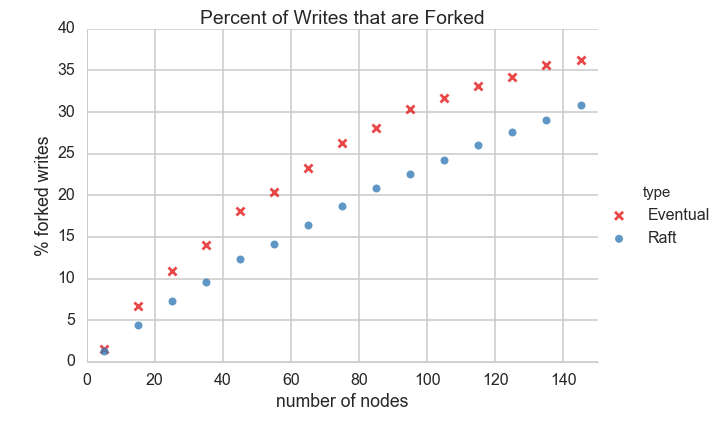
\includegraphics[width=\linewidth]{figures/scaling/forked_writes}
      \caption{Forks in homogenous Raft and eventual consistency systems.}\label{fig:scaling_forked_writes}
    \endminipage\hfill
    \minipage{0.5\textwidth}
      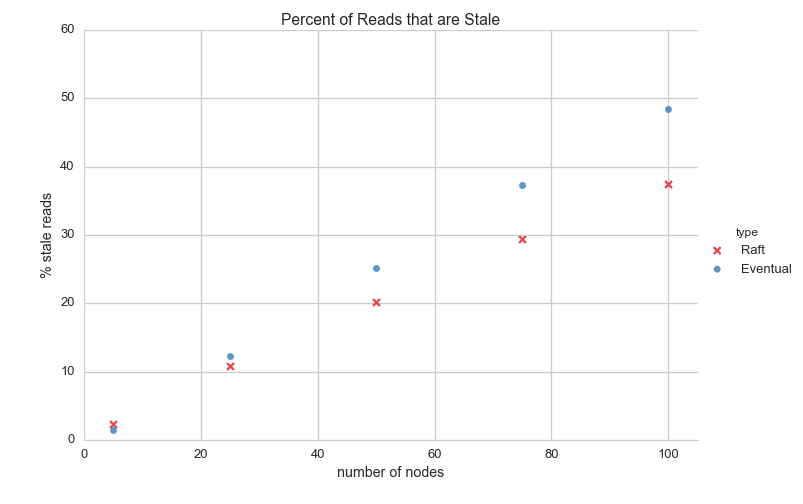
\includegraphics[width=\linewidth]{figures/scaling/stale_reads}
      \caption{Stale reads in homogenous Raft and eventual consistency systems.}\label{fig:scaling_stale_reads}
    \endminipage
\end{figure*}

\section{Proposed Work}

\subsection{Federated Consistency}

\subsection{Hierarchical Consensus}

\subsection{Adaptive Consistency}

\section{Timeline}

\begin{center}
\begin{tabular}{|l|c|}
\hline
Federated Consistency & 2 months \\
Hierarchical Consensus & 3 months \\
Flow File System & 4-5 months \\
Adaptive Consistency & 2-3 months \\
\hline
\textbf{TOTAL} & 11-13 months \\
\hline
\end{tabular}
\end{center}

Paper deadline goals:

\begin{itemize}
\item IEEE International Conference on Distributed Computing Systems, June 2017: Federated Consistency
% http://icdcs2017.gatech.edu/
\item ACM Hot Topics in Storage and File Systems 2017, July 2017: Personal Clouds
% https://www.usenix.org/conferences
\item ACM Principles of Distributed Computing, July 2017: Hierarchical Consensus
% http://www.podc.org/
\end{itemize}


\section{Conclusion}

Insert conclusion here.

\newpage

\appendix
\section{Appendix A: Reading List}
\label{app:readinglist}

\subsection{Consensus}

1) \bibentry{thomas_majority_1979}

2) \bibentry{lamport_paxos_2001}

3) \bibentry{chandra_paxos_2007}

4) \bibentry{lamport_fast_2006}

5) \bibentry{ongaro_search_2014}


\subsection{Consistency}

1) \bibentry{lamport_time_1978}

2) \bibentry{terry_managing_1995}

3) \bibentry{bailis_quantifying_2014}

4) \bibentry{bailis_potential_2012}

5) \bibentry{bermbach_consistency_2013}


\subsection{Replication}

1) \bibentry{stoica_chord:_2001}

2) \bibentry{kubiatowicz_oceanstore:_2000}

3) \bibentry{gray_dangers_1996}

4) \bibentry{venkataramani_operating_2002}

5) \bibentry{almeida_version_2002}



% \newpage

% \section{Appendix B}
% \label{app:cvtdp2r}


\newpage

\bibliographystyle{plain}
\bibliography{prelim}

\end{document}
